% =============================================================================
%  s02_seccion.tex — Sección 2: Desarrollo / Argumentación central
%  Agrega tantos frames como necesites dentro de cada subsección.
% =============================================================================

\section{Marco Teórico; ¿Por qué un Anillo?}

% ───────────────────────────────────────────────────────────────────────────────────────────
\begin{frame}{La \termino{Geometría} de la Ciudad}
  \begin{columns}[T]
    \begin{column}{0.32\textwidth}
      \begin{block}{\scriptsize Creación de los XII Cuarteles (1940)}
        \centering
        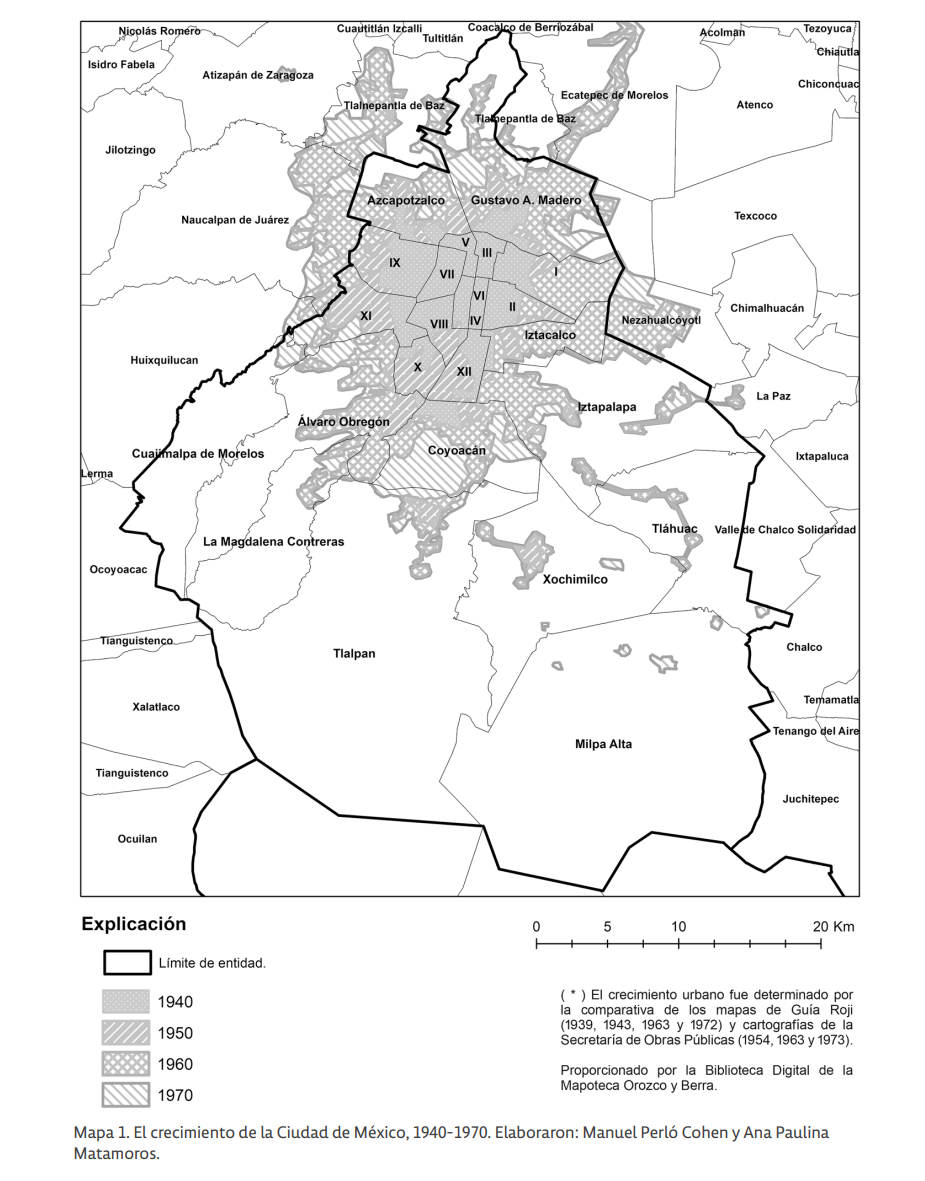
\includegraphics[width=\textwidth, height=3.2cm, keepaspectratio]{img/Uruchurtu1.png}\\[0.3em]
        \scriptsize En los años 40's la Ciudad de México se planeó a través de XII Cuarteles.
        La vía de delimitación fue el Anillo Periférico.
      \end{block}
      \fuentefigura{\cite{padilla2022expansion}}
    \end{column}
    \begin{column}{0.32\textwidth}
      \begin{block}{\scriptsize La Ciudad de Contornos (2020)}
        \centering
        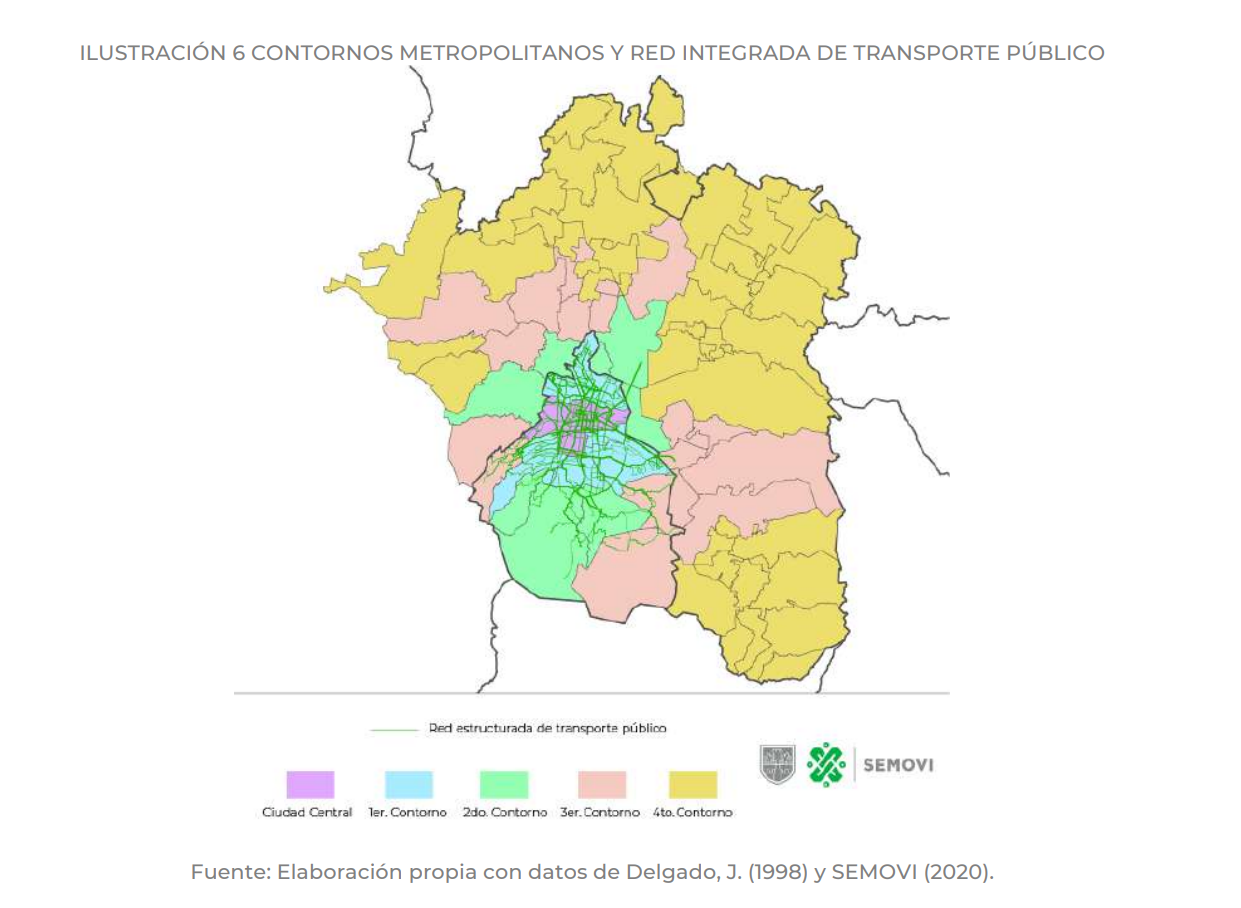
\includegraphics[width=\textwidth, height=3.2cm, keepaspectratio]{img/SEMOVITC.png}\\[0.3em]
        \scriptsize Hoy día la Ciudad de México se divide en 4 contornos, de adentro
        (alcaldías centrales) hacia afuera (alcaldías Periféricas y municipios del EDOMEX).
      \end{block}
      \fuentefigura{\cite{semovi2020diagnostico}}
    \end{column}
    \begin{column}{0.32\textwidth}
      \begin{block}{\scriptsize El Modelo Radial}
        \centering
        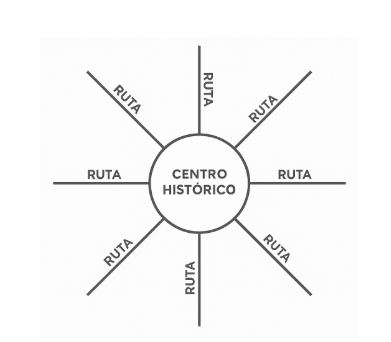
\includegraphics[width=\textwidth, height=3.2cm, keepaspectratio]{img/ETR.png}\\[0.3em]
        \scriptsize La \zmvm sigue una Geometría Radial: las rutas van desde las periferias
        hacia el centro.
      \end{block}
      \fuentefigura{Elaboración Propia con información de: \cite{molinero2002}}
    \end{column}
  \end{columns}
\end{frame}


